\documentclass[aspectratio=1610,10pt,dvipsnames]{beamer}
\usepackage[T1]{fontenc}
\usepackage[utf8]{inputenc}
\usepackage[varg]{txfonts}
\usepackage[french]{babel}
\usepackage{blochsphere}
\usepackage{tikz}
\usetikzlibrary{quantikz}
\usepackage{moreverb}
\usepackage{url} 

\usetheme{Ilmenau}
%%\usetheme{Copenhagen}
%%\usetheme{PaloAlto}
%%\usetheme{Antibes}
%%\usetheme{Warsaw}

\setbeamercovered{transparent}
\setbeamertemplate{footline}[frame number]
%%\usecolortheme[named=green]{structure}

\addtobeamertemplate{footline}{\insertframenumber/\inserttotalframenumber}

\title{Quantum Computing: a quick introduction}
\date{2024}
\institute{CEA}
\author{Philippe DENIEL (philippe.deniel@cea.fr)}

\AtBeginSection[]
{
%%\begin{frame}[plain]
%%%        \usebeamertemplate{section page}
%%%\end{frame}
\begin{frame}{Plan}
\tableofcontents[currentsection]
\end{frame}
}

\begin{document}
\frame{\titlepage}


\section{What is quantum computing?}

\begin{frame}[plain]
\frametitle{A few  citations}

\begin{quotation}{Niels Bohr - }
    Everything we call real is made of things that cannot be regarded as real. If quantum mechanics hasn't profoundly 
    shocked you, you haven't understood it yet.
\end{quotation}

\begin{quotation}{Niels Bohr - }
    Everything we call real is made of things that cannot be regarded as real.
\end{quotation}

\begin{quotation}{Richard Feynmann - }
    If you thought that science was certain - well, that is just an error on your part.
\end{quotation}

\begin{quotation}{Richard Feynmann - }
    I think I can safely say that nobody really understands quantum mechanics
\end{quotation}

\begin{quotation}{Richard Feynmann, 1982 - }
    Nature isn’t classical, dammit, and if you want to make a simulation of nature, you better 	
    make it quantum mechanical
\end{quotation}

\begin{quotation}{Albert Einstein - }
    If you can't explain it simply, you don't understand it well enough
\end{quotation}

\end{frame}

\begin{frame}{What is a computer?}
\begin{tikzpicture}[remember picture, overlay]
\node[left] at (current page.east) 
{
    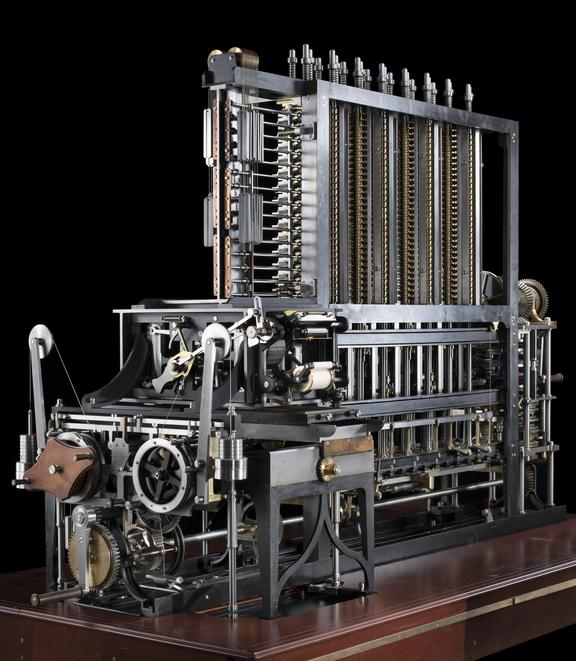
\includegraphics[width=0.25\textwidth]{images/babbage2.jpg}
};
\end{tikzpicture}    
From Wiktionnary, \begin{quotation}
   A computer is a machine that can be programmed to automatically carry out sequences of arithmetic or logical operations (computation). 
\end{quotation}
Several machines are illustrations of this concept:
\begin{itemize}
    \item the \textit{differences engine} by Lord Babbage, fully mechanical,
    \item computers based on electronics, based on Maxwell's theory (and transistors)
\end{itemize}
A Quantum computer is,
\begin{itemize}
    \item a logicam evolution of the concept, this time quantum mechanics is sued to build computatiion devices
\end{itemize}

\end{frame}

\begin{frame}[plain]
\frametitle{Quantum Computing is not really recent}
Le \textit{Quentum Computing} is born in the 80s
\begin{itemize}
   \item a first conferenceabout QC occurend at MIT in 1981
   \item Many theorical studies are made about QC, leading to revolutionnary algorithms
   \begin{itemize}
       \item Shor Algorithm, 1994
       \item Grover Algorithm, 1996
   \end{itemize}
\end{itemize}

QC has very concrete theorical basements
\begin{itemize}
    \item in physics (quantum physics, statistical physics)
    \item in mathematics (linear algebra, hermitian algebra)
\end{itemize}


Real "Quantum Computers" exists for a few years only. 

\end{frame}

\begin{frame}[plain]
\frametitle{Links between Quantum Compurting and Quantum Physics}
\textit{Quantum Computing} is a new paradigm based on Quantum Physics phenomenons:
\begin{enumerate}
    \item superposition,
        \begin{itemize}
            \item QC introduces a \textit{kind of} material paralellism
        \end{itemize}
    \item entanglement,
         \begin{itemize}
            \item couples simpler system in order to build larger systems
         \end{itemize}
    \item interferences,
        \begin{itemize}
            \item make it possible to build unitary operators and measure quantum physics observables
         \end{itemize}
\end{enumerate}
\end{frame}

\begin{frame}{The first quantum revolution}
    Quantum Physics is already there in your everyday life.  
    \begin{itemize}
        \item medicine : MRI, magnetic resonance imaging.,
        \item electronics : Transistors based on tunnel effect, LED,
        \item lasers,
        \item LCD screens,
        \item  photovoltaïcs : photon/matter interaction.
    \end{itemize}
\end{frame}

\begin{frame}{QC and the second quantum revolution}
Quantum Computing belong to the second quantum revolution\\[0.5cm]

 \textbf{QPU}s start appearing on the market. \\[0.5cm]

Several steps are identified
\begin{itemize}
    \item NISQ : \textbf{N}oisy \textbf{I}ntermediate \textbf{S}cale \textbf{Q}uantum
    \item FTQC : \textbf{F}ault \textbf{T}olerant \textbf{Q}uantum \textbf{Q}uantum
    \item LSQ : \textbf{L}arge \textbf{S}cale \textbf{Q}uantum
\end{itemize}
We currently are in the NISQ era. 

\begin{tikzpicture}[remember picture, overlay]
\node[left] at (current page.east) 
{
    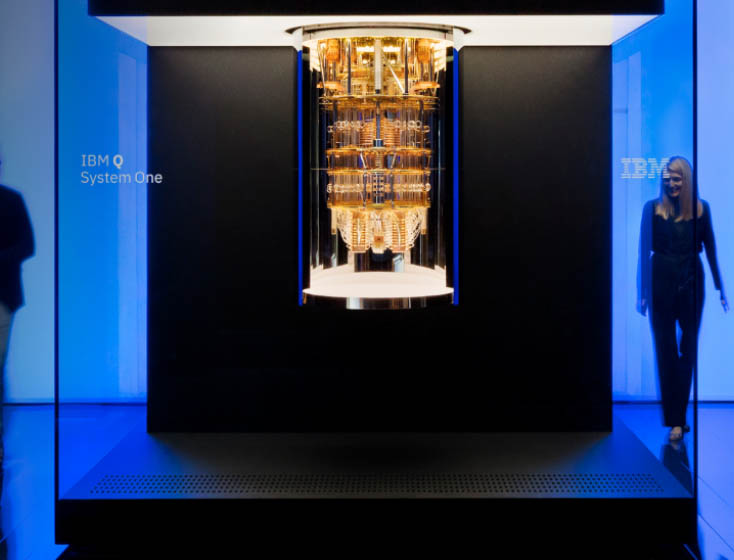
\includegraphics[width=0.25\textwidth]{images/QPU-IBM.jpg}
};
\end{tikzpicture}

\end{frame}

\begin{frame}{What Quantum Computing is not}
QC will never replace HPC
\begin{itemize}
    \item QPUs buold a new HPC paradigm, such as GPUs.
    \item QC is a new weapon in the HPC's armory
\end{itemize}

Beware the "Quantul Hype"!!!!
\begin{itemize}
    \item advertissements, often far from reality
    \item fuzzy articles in general purpose newpapers, 
    \item QC is not "doing $2^n$ computations at the same time", exponential parallelism exists but it does not 
    occur everytime.
    \item  QC  is good to ccaracterize a global property of a known problem
    \begin{itemize}
        \item periodicity of an integer function (Shor)
        \item walking a graph (quantum walks)
        \item locating optima of a quadratic function (QUBO)
    \end{itemize}
\end{itemize}
\end{frame}
\section{A bit of Quantum Physics}

\begin{frame}{The Schrödinger equation}

Quantum Physics describes phenomenons at the scale of atoms and particles\newline


The Schrödinger equation is primarily important
\begin{equation*}
        i\hbar\frac{\partial}{\partial t}\Psi(x,t)=-\frac{\hbar^2}{2m}\nabla^2\Psi(x,t)+V(x,t)\Psi(x,t).
\end{equation*} 
On note que
\begin{itemize}
    \item it takes its value in $\mathbb{C}$, we can notice the $i$ from pure imaginary number on the left handside. 
    \item we notice the $\nabla$ operator from differential geometry, it's used in Maxwell equations
    (electromagnetism) and in Navier-Stokes equation (hydrodynamic)
    \item $\hbar = \frac{h}{2\pi}$ where $h$ is the Planck's constant ($h = 6,62607015.10^{-34} J.s$) 
    \item actions on quantum objects are unitary operators within an Hilber vector space.
\end{itemize}
\end{frame}

\begin{frame}{Consequence of the Schrödinger equation}
Several things result from te Schrödinger equation 
\begin{itemize}
    \item quantum phenomenons take discrete value or \textit{quantas}
    \item quantum objects do not continuously go from one state to another
    \item quantum objects can exist in a superposition of several states at the same time.
    \item quantum objects can simultaneously waves and particles
\end{itemize}
\begin{center}
    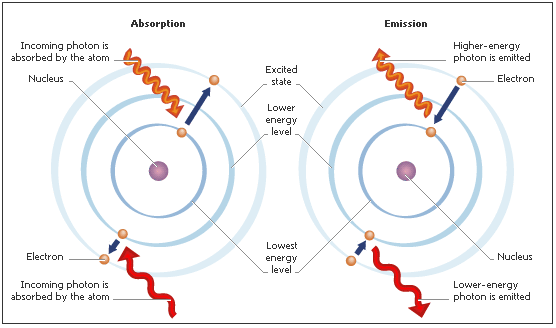
\includegraphics[width=0.50\textwidth]{images/photon.png}    
\end{center}
\end{frame}

\begin{frame}{Superposition}
Quantum objects are linear combinations of basic states, belonging to an orthonormal basis, such as
\begin{equation*}
    \ket{\Psi} = \alpha\ket{0}+\beta\ket{1}+\gamma\ket{2}+\delta\ket{3}
\end{equation*}
Complex coefficients $\alpha$, $\beta$, $\gamma$ et $\delta$ are \textit{complex probabilities}
\begin{itemize}
    \item they respect the normalisation rule$|\alpha|^2+|\beta|^2+|\gamma|^2+|\delta|^2 = 1$
    \item each square of the coefficient module shows the probability to measure the related state (we have a  
    probability $|\alpha|^2$ to see state$\ket{0}$ when observing $\ket{\psi}$
\end{itemize}
\end{frame}

\begin{frame}{Observation and quantum collapse}
In Quantum Physics, observation is a destruction operation, it alters the watched state
\begin{equation*}
    \ket{\Psi} = \alpha\ket{0}+\beta\ket{1}+\gamma\ket{2}+\delta\ket{3}
\end{equation*}
Observing $\ket{\Psi}$ will result in\textbf{collapsing} state $\ket{\Psi}$ on one of the 4~possible states
\begin{itemize}
    \item we see only one of those states, not the 3 other ones
    \item once $\ket{\Psi}$ is collapsed, it won't change anymore. 
\end{itemize}
With Quantum Computing, we build an "intrumented quentum physics experience", we can repeat the experience that builds
 $\ket{\Psi}$ as many times as required
\begin{itemize}
    \item by doing several "shots", we know the probability of each "base state"
    \item \textbf{BEWARE~:} we know the squares of the coefficients's modules (as complex numbers) not the value themselves
    (we mesure $|\alpha|^2$ and not $\alpha$) 
    \item we have no access to the whole information ccarried by  $\ket{\Psi}$
    \item particularily, "phase factors" (written as $e^{i\theta}$) are invisible because they are unitary. 
\end{itemize}
\end{frame}

\begin{frame}{Entanglement}
Entanglement is a very anti-intuitive concept\newline

Einstein did not believed in it, he wrote the famoux EPR (Einstein-Podolsky-Rosen) in 1934\newline

In 1982, the experience by Alain Aspect prooved that entanglement was real, we won the Nobel Price in 2022. \newline

An entangled state groups several particles that should be considered as a single quantum object
\begin{itemize}
    \item when two particles $A$ et $B$ are entangled, whatever acts on $A$ acts on  $B$ too, it actually operates on 
    the entangled system $A \otimes B$
    \item we can't separate $A$ and $B$, they should be handled together
    \item entanglement is no interactation, it is not impacted by distance
    \item in particular, measuring $A$collapses it and collapses $B$ too, simultaneously. 
\end{itemize}
\end{frame}

\begin{frame}{Basements of quantum computing}
Quantum Computing is based on the 3 principles of quantum physics
\begin{itemize}
    \item superposition helps in encoding information in quantum states within several \textit{qubits}
    \item entanglement helps building complex systems made of several qubits
    \item Interference makes it possible to build unitary operation as well as mesure operators. Mesuring always results
    in collapsing the states
\end{itemize}
\end{frame}

\begin{frame}{Concrete mathematical basements}
Quantum physics can be implemented via very concrete mathematics
La physique quantique s'appuie sur un socle mathématique très solide~:
\begin{itemize}
    \item  quabits exist within a 2 dimension $\mathbb{C}$-fied, it is an Hilbert field
    \itemà $n$ qubits systems exist in a Hilbeet field whose dimension is $2^n$
\end{itemize}
Mathematically we can describe
\begin{itemize}
    \item the operators acting on quabits (vectors in a field)
    \item how qubits interact tohether
    \item qubit measurement
    \item formal expression of entanglement
\end{itemize}
Quantum Physics often makes use lots of linear algebra in Hibert fields.
\end{frame}

\begin{frame}{Main ideas expressed here}
Fundamentally, quantum programming is
\begin{itemize}
    \item an intrumented experience of Quantum Physics
    \item smart use of a quantum mechanics phenomenons to accelerate some HPC steps 
    \begin{itemize}
        \item these steps, mapped on QC expeirences, are of complexity NP-C, QC make NP problems reachable by HPC
        \item HPC will always be required to bootstrap QC 
    \end{itemize}
\end{itemize}
Most of the time, QC is good to identift the charactéeristics of a known gloabl property 
\begin{itemize}
    \item given a function $f$,  periodic, what is its period ? (Shor)
    \item given a function $f$  null almost everywhere what are the $x$ such as $f(x) \neq 0$ ? (Grover)
    \item identifying  minima and maxima of quadratic function expressed as matrices (QUBO)
    \item identifying the properties of a graph (MIS, MVC, Clique, MaxCut,...) 
\end{itemize}
\end{frame}



\section{Quantum Gates}

\begin{frame}{Qubits}
Qubit os a quantum system that exists in two possible states  $\ket{0}$ et $\ket{1}$. 
\newline \newline
A subit is a superposition, written as 
\begin{equation*}
    \ket{\Psi} = \alpha\ket{0}+\beta\ket{1}, \alpha \in \mathbb{C}, \beta \in \mathbb{C},  
    \textrm{ avec } |\alpha|^2+ |\beta|^2 = 1
\end{equation*}
for examle $\ket{\Psi} = 0.6\ket{0} + 0.8\ket{1}$ (et on a $0.6^2+0.8^2 = 0.36+0.64=1$)
\end{frame}

\begin{frame}{The Qubit Zoo}
Several kinds of physical qubits can de listed
\begin{itemize}
    \item spin of a particle(encoded on $\ket{UP}$ et $\ket{DOWN}$]
    \item excitation of an electron  (cold atoms, trapped ions=,  NV centers)
    \item supraconducting loops
    \item polarisation of a photon
    \item location of a particle in a system (toplogical qubit)
\end{itemize}
\end{frame}

\begin{frame}{Dirac's notation}
    Base quabits build the canonicam base for $\mathbb{C}^2$, in Direac's notation they are written as
\begin{equation*}
    \begin{split}
        \ket{0} &= \begin{pmatrix} 1 \\ 0 \end{pmatrix} \\
        \ket{1} &= \begin{pmatrix} 0 \\ 1 \end{pmatrix} \\
    \end{split}
\end{equation*}
Which eans that if $\ket{\Psi} = \alpha\ket{0}+\beta\ket{1}$
\begin{equation*}
    \ket{\Psi} = \begin{pmatrix} \alpha \\ \beta \end{pmatrix}
\end{equation*}
\end{frame}

\begin{frame}{One Qubit Gate}
All operator acting on qubits is unitary, which means
\begin{itemize}
    \item it's a matric in $\mathbb{C}^{2 \times 2}$, isomorphic to a  $4\times4$ real matrix, in
    $\mathbb{R}^4$
    \item as an unitary $U$, its  its adjoint matrix is the inverse of $U \times U^{\dag} = \mathbb{I}$ 
    \item it represent a rotation in $\mathbb{C}^2$ which can be seen as a rotation in $\mathbb{R}^4$
\end{itemize}
We have the operators $X$, $Y$ and $Z$
\begin{itemize}
    \item they are dual to Pauli operators from Quantum Physics
    \item they all "almost" dual to $i$, $j$ et $k$ from quaternions in $\mathbb{H}$
\end{itemize}
Every 1 qubit gate can be written as
\begin{equation*}
    U = a\mathbb{I} + bX + cY + dZ, a \in \mathbb{R}, b \in \mathbb{R}, c \in \mathbb{R}, d \in \mathbb{R}
\end{equation*}
\end{frame}

\begin{frame}{Superposition and H Gate}
The H gate, or \textit{Hadamard's gate} helps in building superposed states. \newline \newline
We have the following equations
\begin{equation}
\begin{split}
    H\ket{0} &= \frac{1}{\sqrt{2}}(\ket{0}+\ket{1}) = \ket{+}\\
    H\ket{1} &= \frac{1}{\sqrt{2}}(\ket{0}-\ket{1}) = \ket{-}
\end{split}
\end{equation}
H is a  $2\times 2$ matrix
\begin{equation*}
    H = \frac{1}{\sqrt{2}}\begin{pmatrix}
                           1 & 1 \\
                           1 & -1 \\
                          \end{pmatrix}
\end{equation*}
\end{frame}

\begin{frame}{X gate et qubit flips}
The X gate apparently works like the boolean NOT
\begin{equation*}
    X\ket{0} = \ket{1} \textrm{ et } X\ket{0} = \ket{1}
\end{equation*}
which means that
\begin{equation*}
    \textrm{If } \ket{\Psi} = \alpha\ket{0}+\beta\ket{1} \textrm{ Then } X\ket{\Psi} = \beta\ket{0}+\alpha\ket{1}
\end{equation*}
X is a $2\times 2$ matrix
\begin{equation*}
    X = \begin{pmatrix}
            0 & 1 \\
            1 & 0 \\
        \end{pmatrix}
\end{equation*}
It's important to realize that X is a rotation in $\mathbb{C}^2$ and no bollean operation. It's easy to build a square root 
of X, an "half X rotation" that you need to operate twice to have a complete X. 
Il est important de voir X comme une rotation et pas comme une inversion booléenne, on peut trouver une racine carrée
\begin{equation*}
     \sqrt{X} = \frac{1}{2}\begin{pmatrix} 1+i & 1 - i \\ 1 - i & 1 + i \end{pmatrix}  \textrm{ is such that }
     \sqrt{X}\times \sqrt{X} =  \begin{pmatrix} 0 & 1 \\ 1 & 0 \\ \end{pmatrix} = X
\end{equation*}
\end{frame}

\begin{frame}{Z gate and phase flip}
The Z gate reverses the phases, it reverse the sigh before the $\ket{1}$  component of a state \newline 
\begin{equation*}
    \textrm{Si } \ket{\Psi} = \alpha\ket{0}+\beta\ket{1} \textrm{ alors } Z\ket{\Psi} = \alpha\ket{0}-\beta\ket{1}
\end{equation*}
Z is a $2\times 2$ matrix
\begin{equation*}
 Z = \begin{pmatrix}
            1 & 0 \\
            0 & -1 \\
        \end{pmatrix}
\end{equation*}
The Y gate can be built using X and Z gates
\begin{equation*}
     Y = \begin{pmatrix}
            0 & -i \\
            i & 0  \\
        \end{pmatrix}  \textrm{ et } Y = iXZ
\end{equation*}
\end{frame}

\begin{frame}{This is an (electrical) circuit}
    \centering
    \includegraphics[width=10cm]{images/circuit_électrique.png}
\end{frame}

\begin{frame}{This is no pipe}
    \centering
    
\includegraphics[width=10cm]{images/pipe.jpg}
\end{frame}

\begin{frame}{This is no circuit, this is actually a matrix!}
The following circuit build the famous \textit{EPR} pair
\begin{center}
\begin{tikzpicture}
    \node[scale=1.2] {
        \begin{quantikz}
           & \gate{H} & \ctrl{1} & \qw  & \qw \\
           & \qw      & \targ{}  & \qw  & \qw 
        \end{quantikz}
    };
\end{tikzpicture} 
\end{center}
This circuit is actually depicted by this matrix
\begin{equation*}
    \frac{1}{2}\begin{pmatrix}
                           1  &  0  &  1  &   0  \\
                           0  &  1  &  0  &   1  \\
                           0  &  1  &  0  &  -1  \\
                           1  &  0  &  -1 &   0  \\
                       \end{pmatrix}
\end{equation*}
\end{frame}


\begin{frame}{My first quantum circuit}
Gate based quantum programming builds complex matrices from simpler components.
\begin{center}
 \begin{quantikz}
       \qw  & \gate{H} & \gate{Z} & \gate{H} & \qw
\end{quantikz}
\end{center}
means: apply H, then Z, then H, which in gloabl apply the matrix product $H\times Z \times H$
\begin{equation*}
\begin{split}
    H\times Z \times H &= \frac{1}{\sqrt{2}}\begin{pmatrix}
                           1 & 1 \\
                           1 & -1 \\
                          \end{pmatrix} \times
                           Z = \begin{pmatrix}
                            1 & 0 \\
                            0 & -1 \\
                          \end{pmatrix} \times
                          \frac{1}{\sqrt{2}}\begin{pmatrix}
                           1 & 1 \\
                           1 & -1 \\
                          \end{pmatrix} \\
                        &= \frac{1}{2}\begin{pmatrix}
                                0 & 2 \\
                                2 & 0 \\ 
                        \end{pmatrix} = 
                        \begin{pmatrix}
                            0 & 1 \\
                            1 & 0 \\
                        \end{pmatrix} = X
\end{split}
\end{equation*}
THis shows that this circuit is equivalent to an X gate. 
\begin{center}
 \begin{quantikz}
       \qw  & \gate{H} & \gate{Z} & \gate{H} & \qw  & \textrm{ correspond à   } & \gate{X} & \qw
\end{quantikz}
\end{center}
\textbf{IMPORTANT~:}~Quantum circuit are a smart way of depicting a potentially huge (and unreadable) matrix. They are 
definitely no relatio with circuits involved in electronics. 

\end{frame}

\begin{frame}{Entanglement and CNOT gate 1/2}
The CNOT gate, or CX, intruduces entanglement. It introduces kind of "if-then-else" logic that leads to condutionnl 
statements\newline

CNOT acts on a 2 qubits state, if the first is $\ket{0}$, the second is untouched, but if it is $\ket{1}$, a X gate is 
applied on the second qubit.
\begin{equation*}
    CX\ket{00} = \ket{00}, CX\ket{01} = \ket{01}, CX\ket{10} = \ket{11}, CX\ket{11} = \ket{10}
\end{equation*}
CX is $4 \times 4$ matrix
\begin{equation*}
    CX = \begin{pmatrix} 1 & 0 & 0 & 0 \\ 0 & 1 & 0 & 0 \\ 0 & 0 & 0 & 1 \\ 0 & 0 & 1 & 0 \\ \end{pmatrix}
\end{equation*}
\end{frame}

\begin{frame}{Entanglement and CNOT gate 2/2}
Generically, if $x$ and $y$ are booleans  $(x,y) \in \{0,1\}^2$, then the first qubit $\ket{x}$  does not change while
 $\ket{y}$ becomes $\ket{x \oplus y}$ ($\oplus$ is the boolean XOR)
\begin{center}
    \begin{tikzpicture}
        \node[scale=1.0] {
            \begin{quantikz}
                \ket{x} & \qw & \ctrl{1} & \qw & \qw & \ket{x} \\
                \ket{y} & \qw & \targ{}  & \qw & \qw & \ket{x \oplus y}  
            \end{quantikz}
        };
    \end{tikzpicture}
\end{center}   
CX is a rotation in $\mathbb{C}^4$, isomorphic to a rotation in $\mathbb{R}^8$, we can do "half of it" and so compute a 
square root of CNOT
\begin{equation*}
\sqrt{CX} = \frac{1}{2}
            \begin{pmatrix}
                1 & 0 & 0 & 0 \\
                0 & 1 & 0 & 0 \\
                0 & 0 & 1+i & 1-i \\
                0 & 0 & 1-i & 1+i \\
            \end{pmatrix}   
\end{equation*}
\end{frame}

\begin{frame}{Building the EPR pair}
The EPR pair $\frac{1}{\sqrt{2}}(\ket{00}+\ket{11})$ is an entangled state built by this circuit
\begin{center}
        \begin{tikzpicture}
        \node[scale=1.0] {
            \begin{quantikz}
                & \ket{0} & \gate{H} & \ctrl{1} & \qw  & \qw \\
                & \ket{0} & \qw      & \targ{}  & \qw  & \qw 
            \end{quantikz}
        };
    \end{tikzpicture}
\end{center}
We can compute that
\begin{itemize}
    \item the H gate creates state  $\frac{1}{\sqrt{2}}(\ket{0}+\ket{1})\ket{0} = \frac{1}{\sqrt{2}}(\ket{00}+\ket{10})$
    \item on applique CX operate of each part of the sum and we get 
    $\frac{1}{\sqrt{2}}(CX\ket{00}+CX\ket{10}) = \frac{1}{\sqrt{2}}(\ket{00}+\ket{11})$
\end{itemize}

\end{frame}

\begin{frame}{Controlled gates}
CNOT gate is very important, we can used it to build any other controlled gate
\begin{itemize}
    \item knowing unitary operator $U$, it is applied on the second qubit if the first qubit is $\ket{1}$
    \item recursively, we can build double control... and more!
    \item knwoing square or forth root of $U$ is doable (it a rotation) and important in build $CU$ or $CCU$ gates
\end{itemize}   
\begin{center}
        \begin{tikzpicture}
        \node[scale=0.8] {
            \begin{quantikz}
                 &  \ctrl{1} & \qw  &  & &  \ctrl{2} & \qw    \\
                 &  \gate{U} & \qw  &  & &  \ctrl{1} & \qw    \\
                 &           &      &  &  & \gate{U} & \qw  
            \end{quantikz}
        };
    \end{tikzpicture}
\end{center}
The CCNOT gate, or Toffoli gate is well known
\begin{center}
    \begin{tikzpicture}
        \node[scale=0.8] {
            \begin{quantikz}
                \ket{x} & \qw & \ctrl{1} & \qw & \qw & \ket{x} \\
                \ket{y} & \qw & \ctrl{1} & \qw & \qw & \ket{y} \\
                \ket{z} & \qw & \targ{}  & \qw & \qw & \ket{z \oplus (x \land y)} 
            \end{quantikz}
        };
    \end{tikzpicture}
\end{center}
\end{frame}

\begin{frame}{Key ideas}
Quantum Programming is composing simple unitary operators as building blocks to build bigger and more complex operators
acting on $n$ qubits.
\begin{itemize}
    \item the \textbf{H gate or Hadamard gate} introduces one-qubit superposition
    \item the \textbf{porte X} or NOT gate looks like a boolean NOT but is actually a rotation (like all unitary operators) 
    \item the\textbf{CNOT gate} introduces quantum entanglement and helps building an "if-then-else" logic
\end{itemize}


Quantum Programming is
\begin{itemize}
    \item expressing a known problem as a unitary operator
    \item buold this unitary operator as a circuit
    \item benefit from acceleration (or lesser energy consumption) when executing the circuit
\end{itemize}
Most important: remmber that \textbf{all actions are ALWAYS unitary matrices}
\end{frame}

\section{Algorithmes quantiques}

\begin{frame}{Oracles}
Let  $f$ be an boolean function ~: $f: \{0,1\} \rightarrow \{0,1\} $. 
\newline \newline
 $f$ is integrated in a quantum circuit as a black box named an \textbf{oracle}. \newline
An oracle has to be linear and inversible
\begin{itemize}
    \item the $n$ first qubits carry input data and will not be changed
    \item the other qubits, or \textbf{acillae}, are XOR-d with the result of $f$ on input data
\end{itemize}
\begin{center}
 \begin{quantikz}[thin lines]
    & \ket{x} & & \qw & \gate[wires=2]{O_f} & \qw & \qw & \ket{x} \\
    & \ket{y} & & \qw &                   & \qw & \qw & \ket{y \oplus f(x)}
\end{quantikz}
\end{center}
The same schema operates on $f: \{0,1\}^m \rightarrow \{0,1\}^n, m, n \in \mathbb{N}^* $ \newline
We obtain the oracle $O_f$ pn $m+n$ qubits~~: $m$ inputqubits and $n$ ancillae 
\end{frame}

\begin{frame}{Deustch-Josza algorithm}
Let $f$ be a boolean function ~: $f: \{0,1\} \rightarrow \{0,1\} $, either constant or uniform. \newline
In standard HPC, 2 runs of $f$ are required, while QC only invokes $O_f$ once. 
\begin{center}
 \begin{quantikz}[thin lines]
    & \ket{0} & & \qw & \qw      & \gate{H} & \gate[wires=2]{O_f} & \gate{H} & \meter{} & \qw & \qw  \\
    & \ket{0} & & \qw & \gate{X} & \gate{H} &                     & \qw      & \qw      & \qw & \qw                        
\end{quantikz}
\end{center}
Final state is
\begin{equation*}
    \ket{\Psi_{final}}{\frac{\ket{0}+(-1)^{f(0)+f(1)}\ket{1}}{\sqrt{2}}}\otimes \ket{-}    
\end{equation*}
\begin{itemize}
    \item if $f$ is constant, $f(0) = f(1)$ alors $\ket{\phi_2} =  
                    {\frac{ (\ket{0} + \ket{1})( \ket{0} - \ket{1} ) }{2}} = \ket{+}\ket{-}$
    \item if $f$ is uniform, $f(0) \neq f(1)$ alors $\ket{\phi_2} = 
                    {\frac{ (\ket{0} - \ket{1})( \ket{0} - \ket{1} ) }{2}} = \ket{-}\ket{-}$                
\end{itemize}
by mesuring le first qubit, we get $\ket{+}$ or $\ket{1}$ depending on the properties of $f$. \newline \newline
If a hat contains two balls, each can be back or white, a single shot of Deutsch-Josza tells you if the two balls have the
same colours or different colours. It can be generalised to $n$ qubits.
\end{frame}

\begin{frame}{Bernstein-Vazirini algorithm}
Knowing  $s$ a string of $n$ bits,  we build $f$ by
\begin{equation*}
    \begin{split}
        f & : \{0,1\}^n \rightarrow \{0,1\} \\
          & x \mapsto s \cdot x  = {s_1}{x_1} \oplus {s_2}{x_2} \oplus \cdots \oplus {s_n}{x_n} =
                        {s_1}{x_1} + \cdots + {s_n}{x_n} \textrm{ modulo 2} \\
    \end{split}
\end{equation*}    
We know $f$, can we find $s$ ?
\newline \newline
With a classical approach, at leat $2^{n-1}$ shots should be done in order to build an independant and simple linear
system of equations to be solved to find $s$.
\end{frame}

\begin{frame}{Bernstein-Vazirini's circuit}
\begin{center}
    \begin{tikzpicture}
        \node[scale=0.8] {
        \begin{quantikz}[thin lines]
        & \ket{0}\otimes^n & & \qw & \qwbundle{n} & \gate{H\otimes n} & \gate[wires=2]{O_f} & \qw & \qwbundle{n} & \qw \\
        & \ket{0}          & & \qw & \gate{X}     & \gate{H}          &                     & \qw      & \qw     & \qw 
        \end{quantikz}            
        };
    \end{tikzpicture}
\end{center}
will lead to state
\begin{equation*}
   \ket{\psi} =  \frac{1}{2^n} \sum_{y=0}^{2^{n-1}} \Bigl[\sum_{x=0}^{2^n -1} (-1)^{f(x)+x\cdot y}\Bigr]\ket{y} 
\end{equation*}
Each$\ket{y}$ will have amplitude $\alpha_y = \frac{1}{2^n} \sum_{x=0}^{2^n -1} (-1)^{f(x)+x\cdot y} $ \newline
When $y=s$, $\alpha_s = f(x)+x.s = x.s + x.s = 2x.s$ meaning that $\alpha_s = 2^n / 2^n = 1$ \newline
As the sum of the square of the module of each $\alpha_y$ is 1, all coefficients are null if $y \neq s$, this means 
that $\ket{\psi}= \ket{s}$ 
\newline
We know $s$ with \textbf{a single} invocation of the oracle. 
\end{frame}

\begin{frame}{Shor algorithm - raw idea}
Let $N$ be a very large integer, written as the priduct of 2 factors... What are those factors?\newline \newline
Let $a$ and $r$ be 2 integers such as  $a^r \equiv 1 [N]$ so $a^r -1 \equiv 0 [N]$ \newline \newline
If $r$ is even, then $r = 2p$ and  $a^{2p} - 1 = (a^p-1)(a^p+1) \equiv 0 [N]$ \newline \newline
So, it exists an integre $k$ such as $(a^p-1)(a^p+1)=kN$ \newline \newline
Computing the largest common divisor of $N$, $(a^p-1)$, $(a^p+1)$ identifies a factor of $N$ \newline \newline
This last operation is easy with HPC (for example by using Euclide algorithm). 
\end{frame}

\begin{frame}{Algorithme de Shor - period search}
Knowing $N$, for all integers $a$ lower than  $\sqrt{N}$ we build the function
\begin{equation*}
    f_a: k \mapsto a^k \textrm{ modulo } N
\end{equation*}
If we find an integer $r$ such as $f_a(r) = a^k = 1$ then $f_a(p+r) = a^p a^r = 1$ and then $f_a$ est r-periodic. 
\newline \newline
The quantum part of the algorithm
\begin{itemize}
    \item takes a value $a$
    \item identify if $f_a$ has a period $r$, if $r$ is even, we won the price!
\end{itemize}
This part uses
\begin{itemize}
    \item a quantum circuit inspired bu the Simon algorithm, which find the period of a boolean function
    \item Quantum Fourier Transform (QFT) or Quantum implementation of Discrete Fourier Transform.
\end{itemize}
\end{frame}

\begin{frame}{Reminder- Discrete Fourier Transform (DFT) - Definition}
Classical Fourier transform associe a function $f$ with
\begin{equation*}
    \hat{f}: \mathbb{R} \rightarrow{} \mathbb{C}, 
    \hat{f}(x) = \int_{-\infty}^{+\infty} f(x) e^{-ixy}  \,dy
\end{equation*}
sometimes written with an explicity "frequency" variable
\begin{equation*}
    \hat{f}(\nu) = \int_{-\infty}^{+\infty} f(t) e^{-2i\pi \nu t}  \,dt
\end{equation*}
If $(s_n)_{0\le n < N}$ is a seri of $N$ values, we can define the discrete Fourier transform by writting, 
$(\hat{s}_n)_{0\le n < N}$ comme la suite de valeurs
\begin{equation*}
    0 \le n < N, \hat{s}_n = \sum_{k=0}^{N-1}s_k.e^{-2i\pi\frac{kn}{N}}
\end{equation*}
\end{frame}

\begin{frame}{Reminder - Discrete Fourier Transform (DFT) - Vandermonde Matrix}
The DFT can be expressed as matrix, known as the Vandermonde matrix
    \begin{equation*}
    QF_n = \frac{1}{\sqrt{N}} W_N = \frac{1}{\sqrt{N}} 
    \begin{pmatrix}
        1       & 1                 & 1                  & \cdot  & 1                        \\
        1       & \omega_{N}       & \omega_{N}^2        & \cdots & \omega_{N}^{N-1}         \\
        \vdots  & \vdots           & \ddots              & \vdots & \ddots                   \\
        1       & \omega_{N}^{N-1} & \omega_{N}^{2(N-1)} & \cdots & \omega_{N}^{(N-1)(N-1)}  \\
    \end{pmatrix}
\end{equation*}
\textbf{Example~:~}with 3 qubits, we'll get the following $8 \times 8$ matrix 
\begin{equation*}
    QF_8 = \frac{1}{\sqrt{8}}\begin{pmatrix}
        1 & 1        & 1        & 1        &  1       & 1        & 1        & 1        \\
        1 & \omega   & \omega^2 & \omega^3 & \omega^4 & \omega^5 & \omega^6 & \omega^7 \\
        1 & \omega^2 & \omega^4 & \omega^6 & 1        & \omega^1 & \omega^4 & \omega^6 \\
        1 & \omega^3 & \omega^6 & \omega   & \omega^4 & \omega^7 & \omega^2 & \omega^5 \\
        1 & \omega^4 & 1        & \omega^4 & 1        & \omega^4 & 1        & \omega^4 \\
        1 & \omega^5 & \omega^2 & \omega^7 & \omega^4 & \omega   & \omega^6 & \omega^3 \\
        1 & \omega^6 & \omega^4 & \omega^2 & 1        & \omega^6 & \omega^4 & \omega^2 \\
        1 & \omega^7 & \omega^6 & \omega^5 & \omega^4 & \omega^3 & \omega^2 & \omega^1 \\
    \end{pmatrix} \textrm{ avec } \omega = e^{\frac{2i\pi}{8}}
\end{equation*}
This matrix is unitary. 
\end{frame}

\begin{frame}{QFT Circuit}
The circuit that implement the Vandermonde matrix is based on this mathematical property\newline \newline
\begin{equation*}
    QF_n \times \ket{k} =  \frac{1}{\sqrt{2^n}} \sum_{j=0}^{2^{n}-1} e^{-2i\pi\frac{kj}{2^n}} \ket{j}
                        =  \frac{1}{\sqrt{2^n}} \bigotimes_{j=0}^{n}(\ket{0} + e^{2i\pi\frac{k}{2^j}} \ket{1} )
\end{equation*}
\begin{center}
\begin{tikzpicture}
   \node[scale=0.8] { 
\begin{quantikz}
     & \qw      & \ctrl{4}& \qw           & \qw    & \qw & \qw        & \qw      & \ctrl{3}   & \qw        & \qw
     & \qw & \qw            & \qw  & \qw  & \qw      & \ctrl{1} & \gate{H} & \qw \\
     & \qw      & \qw     & \ctrl{3}      & \qw    & \qw & \qw        & \qw      & \qw        & \ctrl{2}   & \qw
     & \qw & \qw            & \qw  & \qw  & \gate{H} & \gate{R_2} & \qw & \qw \\
              &          & \vdots     &            & \vdots &     &            &          &            &            &  
     &     & \vdots         &      &      &          &           \\
     & \qw      & \qw        & \qw        & \qw    & \qw & \ctrl{1}   & \gate{H} & \gate{R_2} & \gate{R_3} & \cdots  
     & \qw & \gate{R_{n-1}} & \qw  & \qw  & \qw      & \qw  & \qw  & \qw   \\
     & \gate{H} & \gate{R_2} & \gate{R_3} & \cdots & \qw & \gate{R_n} & \qw      & \qw        & \qw        & \qw 
    & \qw  & \qw            & \qw  & \qw  & \qw & \qw & \qw & \qw
\end{quantikz}
    };
\end{tikzpicture}
\end{center}
\end{frame}

\begin{frame}{Quantum implementation of the Shor algorithm}
The quantum part is written as
\begin{center}
 \begin{quantikz}
  & \ket{0} & \gate{H} & \gate[wires=6]{O_f} & \qw & \qw      & \gate[wires=3]{QF_N^{-1}} & \qw & \meter{} & \qw \\ 
  & \ket{0} & \gate{H} &                     & \qw & \qw      &                           & \qw & \meter{} & \qw \\
  & \ket{0} & \gate{H} &                     & \qw & \qw      &                           & \qw & \meter{} & \qw \\             
  & \ket{0}   & \qw    &                     & \qw & \meter{} & \qw                       & \qw & \qw      & \qw \\
  & \ket{0}   & \qw    &                     & \qw & \meter{} & \qw                       & \qw & \qw      & \qw \\
  & \ket{0}   & \qw    &                     & \qw & \meter{} & \qw                       & \qw & \qw      & \qw  
\end{quantikz}
\end{center}   
Where $O_f$ is an oracle that implements $f(x) = a^x$
\end{frame}


\section{Analogic Quantum Computing}

\begin{frame}{Even more maths...}
The maths behin Analogic Quantum Computing (AQC) reside in the theory of complexity\newline

In a nutshell:
\begin{itemize}
    \item some "difficult" problems can be mapped as a quantum physics experiment
    \item when solving a difficult problem in a computation, we first translate it to turn it into
    one of the problems that the AQC can solve
    \item we run sevceral shots of the experiment on AQC to get a result
    \item we translate the result back into a solution of the initial problem
\end{itemize} 


Parmi les implémentations analogiques, on trouve dans le paysage actuel~:
Within the available AQC devices, and the addressable "difficult" problems, we find
\begin{itemize}
    \item supraconductionf loops in D-Wave hardware, addressing the QUBO problem
    \item cold atoms in Pasqal Hardware, addressing the MIS problem
    \item Photonics in Quandela hardware, able to compute the permaent of a matrix
\end{itemize}
\end{frame}

\begin{frame}{P and NP}
In the complexity theory, several classes of problems's complexity exiist
\begin{itemize}
    \item \textbf{P class} problems can be solved by HPC systems, they require a time to solution  varying exponentially
    with the size of the proble
    \item \textbf{NP class} problems are \textit{non-deterministic polynomial} problems, the time to solution is much 
    larger than polynomial, but checking that a candidate for a solution is an actual solution can be checked in a time
    which polynomially depends on the size of the problem. 
\end{itemize}


\textbf{BEWARE}: NP \textbf{does not mean} non-polynomial (it's quite a bad acronyl).
\end{frame}

\begin{frame}{P and NP: examples}
 P problems are addressable by regular HPC 
 \begin{itemize}
     \item computing the gcd and lcm of two very large numbers (Euclide's algorithm)
     \item inverting a matrix (Gauss's algorithm)
     \item identifying is a number is prime or not (AKS algorithm)
 \end{itemize}
NP problem: factorization of the product of two large prime numbers
 \begin{itemize}
     \item I gave you $62062883$, it's a product of two prime numbers... which ones?
     \item It's complicated... the time to solution does not vary polynomially with the number of digits
 \end{itemize}
 I make the asumption that $62062883= 7877 \times 7879$
 \begin{itemize}
     \item it's a potential solution, let's check it!
     \item checking it is fast... we do a mulitplication (which is clearly a polynomial problem)
 \end{itemize}
Factorization is a typical NP problem
\end{frame}

\begin{frame}{The Complexity Zoo}
\centering
    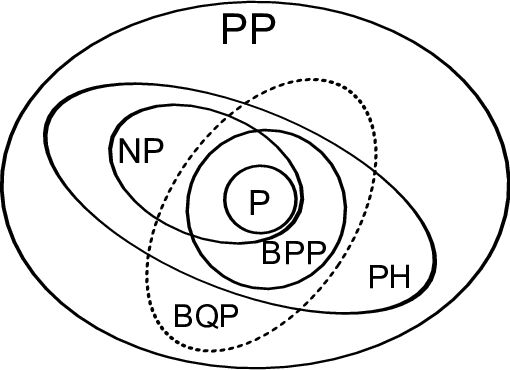
\includegraphics[width=9cm]{
        images/A-diagram-for-the-relations-between-complexity-classes-P-NP-PH-BPP-PP-and-BQP-Note.png}
\end{frame}

 \begin{frame}{NP Complete problems - Cook's theorem}
By definition, a \textbf{NP-hard} problem is so that any NP problem can be translated into this problem. By solving it,
you solve any NP problem. \newline \newline

\textbf{Definition:~} A problem which is both NP and NP-hard is \textbf{NP-Complete}. \newline \newline

The Cook's Theorem (demonstrated in 19771) styates that NPC problems exis, and that converting a NP problem into a NPC one
in a probem whose complexity is of class P (addressable by HPC). \newline \newline

Many NP-Complete probems have been identified (QUBO, Travelling Salesperson (TSP), SAT, MIS, ...), in 1972 the
Karp's list shows 21 of them
\end{frame}

\begin{frame}{Karp's list 1/2}
In 1972, right after the demonstration of the Cook's theorem in 1972, Karp lists 21 NP-Complete problems.
\begin{itemize}
    \item SATISFIABILITY : The SAT problem, the basement of Cook's demonstration
    \item CLIQUE : detecting a "clique" (similar to a social network community) in a graph
    \item SET PACKING 
    \item VERTEX COVER 
    \item SET COVERING
    \item FEEDBACK ARC SET 
    \item FEEDBACK NODE SET 
    \item DIRECTED HAMILTONIAN CIRCUIT 
    \item UNDIRECTED HAMILTONIAN CIRCUIT
    \item INTEGER PROGRAMMING 
    \item 3-SAT 
     \item CHROMATIC NUMBER : finding the "chromatic number" for a graph
\end{itemize}
\end{frame}

\begin{frame}{Karp's list 2/2}
\begin{itemize}
    \item CLIQUE COVER 
    \item EXACT COVER
    \item MATCHING à 3 dimensions 
    \item STEINER TREE 
    \item HITTING SET 
    \item KNAPSACK 
    \item JOB SEQUENCING 
    \item PARTITION 
    \item MAX-CUT 
    \item QUBO
    \item TSP: Traveling Sales Person
\end{itemize}    
\end{frame}

\begin{frame}{QUBO and Simulated Annealing}
\textbf{Q}uadratic \textbf{U}nconstrained \textbf{B}inary \textbf{O}ptimisation focuses on finding optimum of a 
quadratic function (expressed as a real matrix) whose input is a binary vector.
\newline

QUBO is NPC, but it can be approximated since 1984 by textit{Simulated Annealing} method. The algorithm's name 
derive from metallurgy. 
\newline

Simulated Annealing derives from Metropolis-Hastings algorithm, which focuses on thermodynamics. Many implementation
exists (including Mathematica). Its existence since a long time explains why so many "convert to QUBO" methods exist
when it comes to solving NPC problems
\newline

QUBO is natively implented by D-Wave hardware which is capable of providing exact solution of QUBO. 
\end{frame}

\begin{frame}{Le problème Max-Cut 1/2}
Knowing a graph $G=(V ; E)$, made of vertices connected by edges, we want to do the \textit{Maxium Cut}: separate the 
set of vertices $V$ in two complementary parts $V_1$ and $V_2$, so that the set of edges connecting vertices from
$V_1$ and $V_2$ is the largest one. 
\newline

MaxCut can be enhanced by adding \textit{weights} on each edge. It then possible to define a global weight associated with 
a cut. MaxCut will then try to find the cut with the highest global weight.
\centering
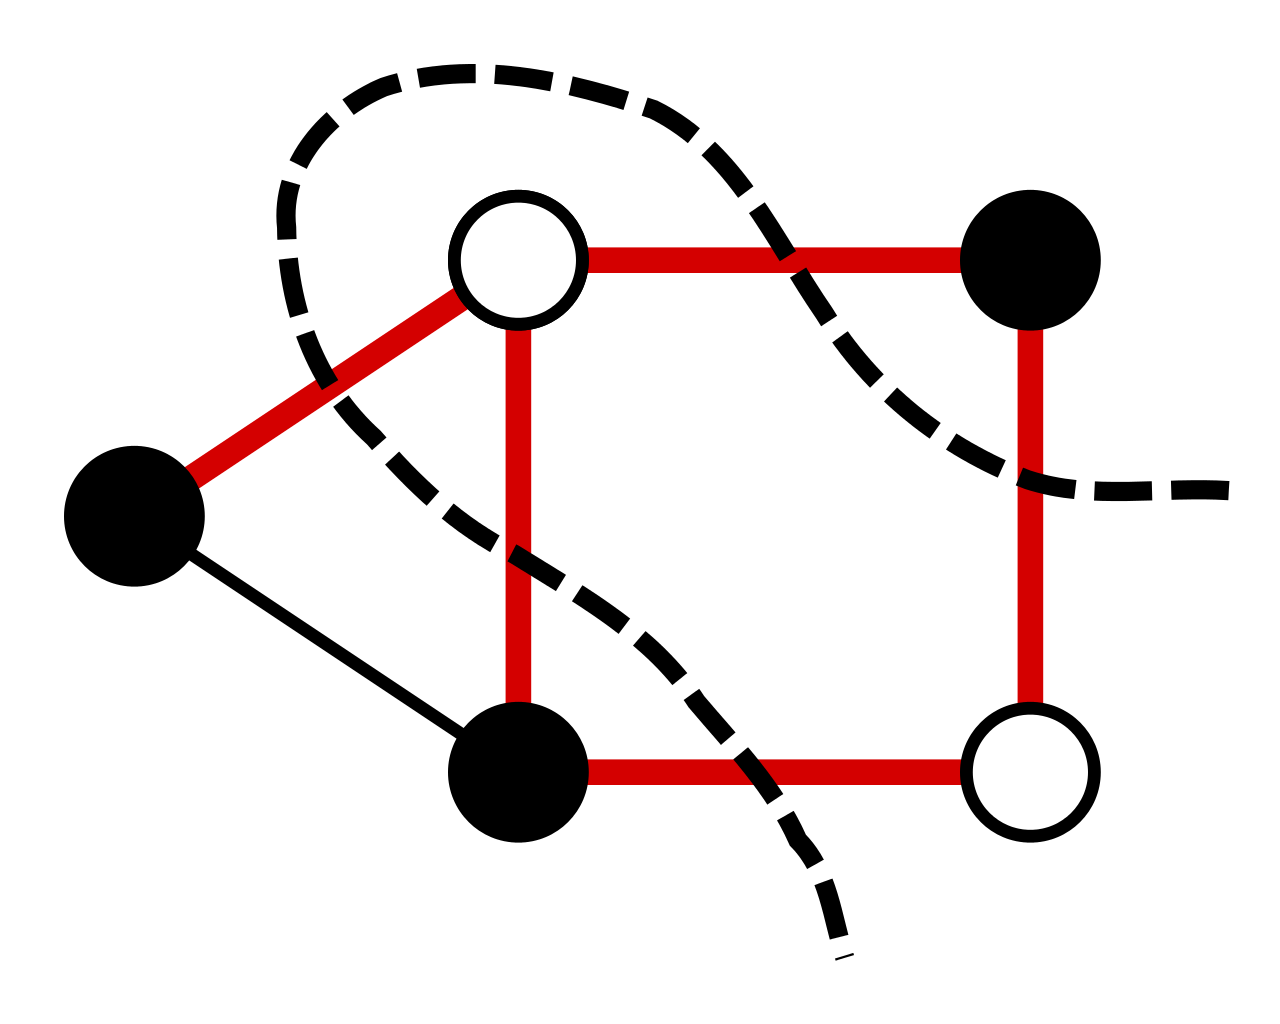
\includegraphics[width=7cm]{images/Max-cut.svg.png}
\end{frame}

\begin{frame}{Le problème Max-Cut 2/2}
\textbf{Remark:} We can define Mincut in a completely similar way.

MaxCut, and the discovery of a maximum cut in a graph is associated with:
\begin{itemize}
    \item decision making problem~: knowing a grap $G$, is there is an integer $k$ such as a cut whose weight is at least $k$
    \item optimisation problem : knowing a graph $G$, find the cut with the highest cut
\end{itemize}

MaxCut has complexity P if the involved graph is \textit{planar} (its dimension is 2); \newline


As graph become more complex, MaxCut is NP-Complete (both NP and NP-hard)
\end{frame}

\begin{frame}{The MIS problem}
Knowing a graphe $G = (V ; E)$, what is the largest set of \textit{independent} vertices, such no edge exist between
any two different elements of this \textit{Maximum Independent Set}.

Sometimes, several different solutions exist 
Il existe souvent plusieurs solutions à ce problème.
\newline

MIS are dominants subsets. A subset of vertices $S$ of a graph is dominant is any vertex is either in $S$, or connected 
(neighbour) to a element in $S$. MIS arte the largets dominant subsets.

\centering
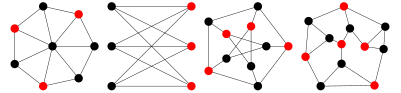
\includegraphics[scale=0.8]{images/MaximumIndependentSet_1000.png}
\end{frame}

\begin{frame}{The MVC problem}
MVC stands for \textit{Maximum Vertex Cover}, it is dual with the MIS problem. 

A cover of vertices is a subset of vertices, it is defined as \textit{transversal} in $G$ if any edge in $E$ connects
to at least one element in the cover. MVC aims to find the smallest transveral cover. 
\newline

Analogy: edges are corridors, verices are "crossroads", where should I installed cameras in order to watch all the 
corridors?

\centering
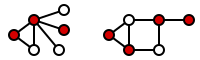
\includegraphics[scale=1.0]{images/Vertex-cover.svg.png}
\end{frame}

\begin{frame}{The SAT problem}
SAT is involved in Cook's theorem's demonstration. Knowing boolean (true or false) variable, we can design a 
\textit{proposition}: a formula using this variables with logicial AND ($\land$) and OR ($\lor$) operator. 
\newline
SAT problem asks this : knowing a proposition, does it have solution? It's not aabout finding solution or counting solutions,
it about knowing if a solution exists. This is why it's call \textit{boolean satisfiability}.
\newline
Example:  $(p\land q)\lor \lnot p$ has result $true$ if $p$ is $false$, with any value for $q$, it can be \textbf{satisfied},
but $(p\land \lnot p)$ has no solution, it can't be satisfied. 

SAT is P with simple proposition, when the proposition's \textit{atoms} involve only two variables, it's 2-SAT. 2-SAT is P.

3-SAT is NP-Complete. Any larger SAT problem can be converted into 3-SAT by increasing the number of variables. 

\end{frame}

\begin{frame}{NP conversion: solving MacCut with QUBO 1/2}

Let's consider this graph with 4 fours and weighted edges.

\centering
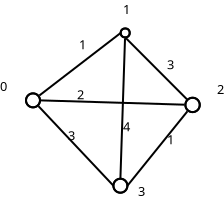
\includegraphics[scale=0.7]{images/graph4pt.png}
\end{frame}

\begin{frame}{NP conversion: solving MacCut with QUBO 2/2}
We can translate the graph into its \textit{connectivity matrix} whose coefficients  $w_{ij}$ are defined by
\begin{itemize}
    \item 0 if $i = j$ 
    \item the weight of the edge connecting  if $i \neq j$ and an efge exist
    \item 0 if no edge exist between nodes $i$ and $j$
\end{itemize}
In our exqmple, we'll build this matrix
\begin{equation*}
 W = \begin{pmatrix}
         0 & 1 & 2 & 3 \\
         1 & 0 & 3 & 4 \\
         2 & 3 & 0 & 1 \\
         3 & 4 & 1 & 0 \\
     \end{pmatrix}    
\end{equation*}
Knowing a graph cut, input binary $b$ has coefficients $b_i$: $1$ if node $i$ is in the cut, 0 otherwise.
Solving MaxCut can be reduced as solving QUBO using the quadratic function associated with the connectivity matrix.
We'll look for the maximum. 
\end{frame}

\begin{frame}{NP conversion: solving 3-SAT with MIS 1/3}
3-SAT can be solved via a MIS problem. 

Let's consider a conjonctive and normal propositiion involving $n$ variables and $m$ clauses.  

\begin{itemize}
    \item for each clause, a small 3 vertices graph is built, each vertex is a variable or the negate of a variable
    \item those small graph are linked by connected a variable in a 3 vertices graph with its negate in another
    3 vertices graph
\end{itemize}
Example: let's consider  $\lnot x_1 \lor x_2 \lor x_3$, it will be depicted by this graph


\centering
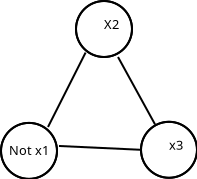
\includegraphics[scale=0.25]{images/Clause3SAT.png}
\end{frame}

\begin{frame}{NP conversion: solving 3-SAT with MIS 2/3}
We connect sub-graphes together by connected $v$ with $\lnot v$

Let's consider
suivante
\begin{equation*}
    (x_1 \lor x_2 \lor x_3) 
    \land (\lnot x_1 \lor x_2 \lor x_3 ) 
    \land (x_1 \lor \lnot x_2 \lor x_3 )
    \land (\lnot x_1 \lor x_2 \lor \lnot x_3 )
\end{equation*}
\centering
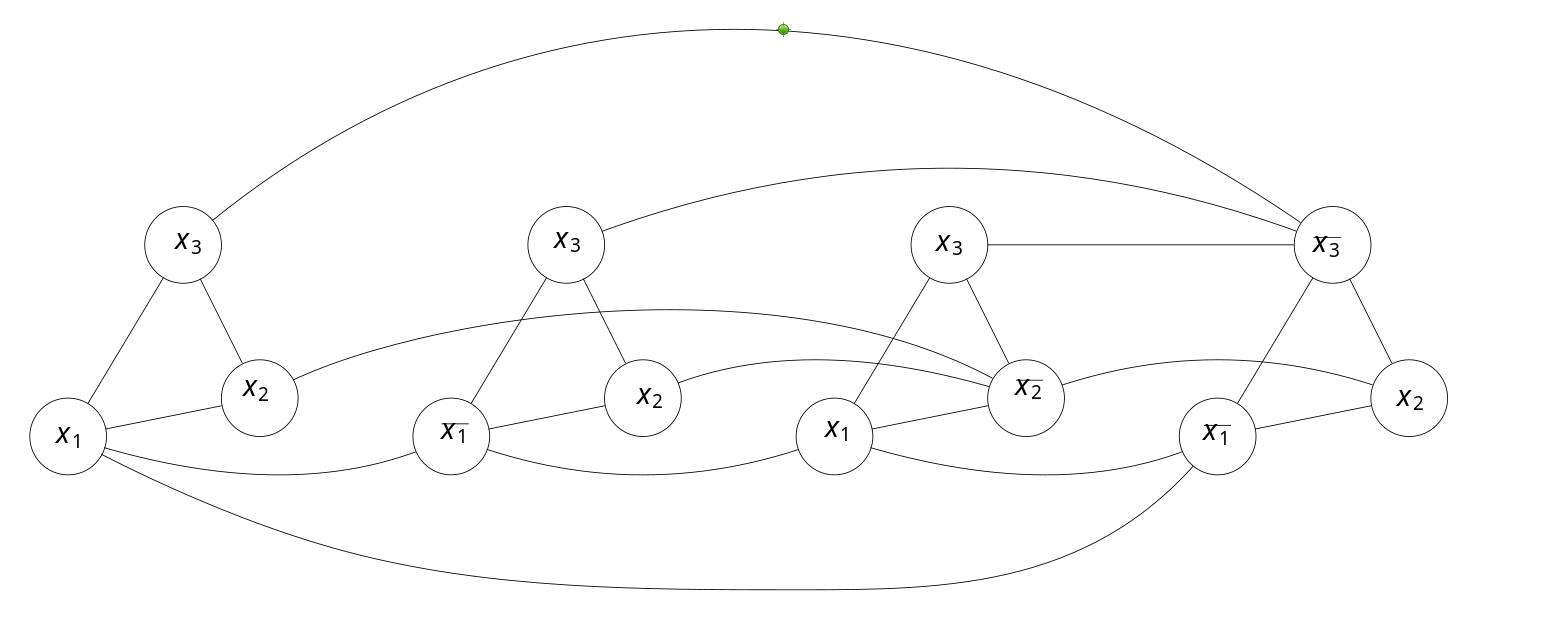
\includegraphics[scale=0.25]{images/Graphe-Clause3SAT.png}
\end{frame}

\begin{frame}{NP conversion: solving 3-SAT with MIS 3/3}
By solving MIS on the resulting graph, we can evaluate the size of this maximum set and compare it to the number of clauses
within the original proposition. If values are the same then the proposition can be satisfied. 


If the MIS size is smallest than the number of clauses, then the proposition can't be satisfied.
\end{frame}

\begin{frame}{NP problems are everywhere}
NP problem are very common in graph theory or in optimisation related problems.

They are often "simple to describe" but "hard to solve".
\begin{itemize}
    \item Traveling Sales Person (TSP) is very interesting for logistics 
    \item Clique problem is very interesting for Social Networks: cliques describe users's community
    \item Many optimisations problem, involving \textit{cost functions}, can be solved as a QUBO
    \item MaxCut is associated with decision making algorithms
\end{itemize}

If any "NP to NPC" conversion is P (Cook's theorem), designing this conversion is very difficult. Many conversion to 
QUBO exist, because QUBO could be approximated since 1984 and was an early point of interest. 
\end{frame}


\begin{frame}{Back to the MIS problem}
The Pasqal hardware can natively address the \textit{Maximum Independant Set} (MIS) problem
\begin{itemize}
    \item let's consider a graph $(G ; E)$
    \begin{itemize}
        \item $G$ is a set of points, or \textit{vertices} in a $n$ dimensions field
        \item $E$ is a set of segments connecting two vertices, or \textit{edges}
    \end{itemize}
    \item we look for the largest set(s) of vertices that are not connected (no edge exist between any two points
    in the MIS)
\end{itemize}

With pasqal hardware, a hardware constraint exist: the graph should be \textit{Unitary Disk Graphs} (UDG), associated 
with a \textit{radius} $R$
\begin{itemize}
    \item vertices whose distance is lower than $R$ are necessarily connected
    \item if two vertices are connected (an edge exists) then the distance between them is lower than $R$
\end{itemize}

This MIS problem is dual to the \textit{Minimum Vertices Cover} (MVC)
\begin{itemize}
    \item in MVC, we want to identfy the smallest set of vertices where "cameras" should be places to see all of the
    edges within a graph.
    \item we can demonstrated that MVC and MIS have no common points and their union is the whole graph.
\end{itemize}
\end{frame}    

\begin{frame}{Pasqal hardware: the physics behind the stage}
The Pasqal system  uses some Quantum Physics phenomenons, which can be mapped to MIS
\begin{itemize}
    \item monovalent (only one electron) Rubidiu atoms are emitted in a void chamber, lasers slow them down and
    place them as "optical tweezers"
    \item the lowest highest excitation level of the electron implement the states $\ket{0}$ and $\ket{1}$
    \item atoms are entangled by thee \textit{Rydberg blocade} mechanism
    \item atoms whose state is $\ket{1}$ can be jected (but we knwow where they have been placed)
    \item with a special camera, remaining atoms are seen using fluorescence 
\end{itemize}
Meanwhile
\begin{itemize}
    \item Atoms have to be within a \textit{Rydberg Radius} in order to be entangled
    \item entangled atoms are in global state $\frac{1}{\sqrt{2}}(\ket{01}+\ket{10})$
\end{itemize}
\end{frame}

\begin{frame}{The Pulser API is not user friendly}
The Pulser API is kind of "control command" related API
\begin{itemize}
    \item it locates the atoms on a grid
    \item it sets the Rydberg Radius by tweaking the correct laser frequencies
    \item it sets the shape of the laser wavelenghts (or \textit{pulses}) used to excitate the atoms  
    \item many shots and related observations are done
\end{itemize}
Pulser does not actual define a "program", it's an advanced toolkit that program the experiment environment for the 
Pasqal system
\end{frame}

\begin{frame}[fragile]
\frametitle{Code sample - Initialisation}
The init of the Pulser python framework looks like this
\newline
\begin{verbatim}
import numpy as np
from pulser import Pulse, Sequence, Register
from pulser_simulation import Simulation
from pulser.devices import MockDevice
from pulser.waveforms import RampWaveform, ConstantWaveform

import matplotlib.pyplot as plt
import qutip
\end{verbatim}
\end{frame}

\begin{frame}[fragile]
\frametitle{Code sample - Graph descriptio,}
\begin{verbatim}
# Define a dictionary where each key is the name of the qubit,
# and each value is the qubit's position (in um)

qubit_positions = {
    'q0': (0, 0),
    'q1': (3, 5.2),
    'q2': (6, 0),
    'q3': (9, -5.2)
}
\end{verbatim}

Ce dictionnaire est ensuite transformé en registre.
\\
\begin{verbatim}
# Arrangements of qubits on the machine are called a register
# Define a register in Pulser by passing the qubit dictionary
reg = Register(qubit_positions)
reg.draw()
\end{verbatim}
\end{frame}

\begin{frame}[fragile]
\frametitle{Set the Graph Radius / Rydberg Radius}
\begin{verbatim}
# Define the maximum Rabi frequency via a blockade radius
blockade_radius = 8.7
Omega_max = MockDevice.rabi_from_blockade(blockade_radius)

# Visualize the edges induced by the chosen blockade radius
reg.draw(blockade_radius=blockade_radius)
\end{verbatim}
\begin{center}
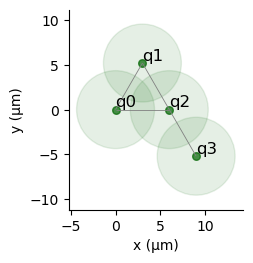
\includegraphics[scale=0.60]{images/reg3.png}
\end{center}

\end{frame}

\begin{frame}[fragile]
\frametitle{Define laser pulses}
\begin{small}
\begin{verbatim}
# A Sequence is the object that contains all
# the info about the quantum evolution
seq = Sequence(reg, MockDevice)

# Now we want to fill the channel with pulses 
# First we need to define the waveforms for the pulses
# First ramp
omega_wf_1 = RampWaveform(300, 0, Omega_max) 

#arguments are duration (ns), detuning (rad/us)
delta_wf_1 = ConstantWaveform(300, -40) 

first_pulse = Pulse(omega_wf_1, delta_wf_1, 0)
seq.add(first_pulse, 'ch')
seq.draw()
\end{verbatim}
\end{small}
\end{frame}

\begin{frame}{Shapes of the wavelengths}
The laser pulses will look like this
\begin{center}
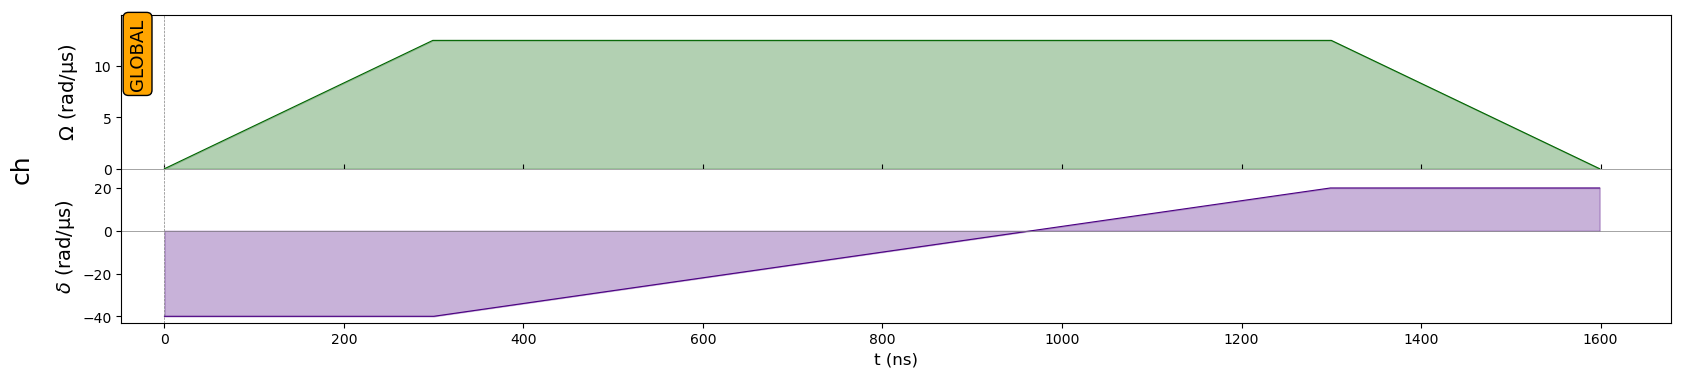
\includegraphics[scale=0.30]{images/seq1.png}
\end{center}
\end{frame}

\begin{frame}[fragile]
\frametitle{Pulser - end of code}
\begin{verbatim}
# The sequence is ready now for simulation

sim = Simulation(seq)
results = sim.run()

# The result can be sampled
samples = results.sample_final_state(10000)

# And the sampling can be visualized
plt.bar(samples.keys(), samples.values())
\end{verbatim}
\end{frame}

\begin{frame}{Results}
We finally get the final result
\begin{center}
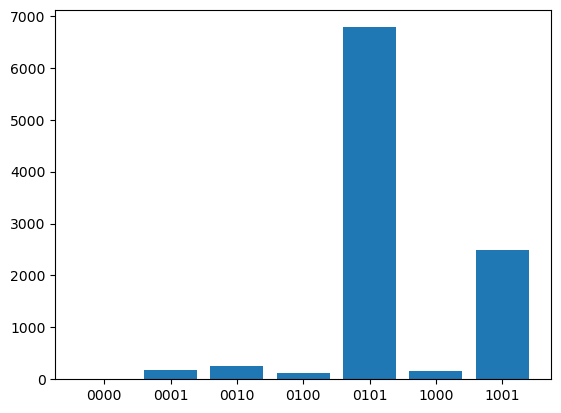
\includegraphics[scale=0.5]{images/histo1.png}
\end{center}
On voit deux solutions : $\ket{0101}$ et $\ket{1001}$. ce sont les solutions du problème MIS.
\end{frame}

\begin{frame}{AQC middle is a requirement}
AQC devices are less sensitive to noise or decoherence, when compared to gate based machines, but the interface operates
at a very low level
\begin{itemize}
    \item pieces of middleware are required to translate a user's NP problem into MIS
    \item pieces of middleware are required to translate a MIS input into a Pulser experiment
\end{itemize}
One of the challenges to future AQC systems will be related to this software integration, mixing HPC and QC since
HPC systems will do all of the "translate stuff". Many things are still to be done. 
\end{frame}


\section{Other QC related topics}

\begin{frame}{Post Quantum Cryptography}
Post Quantum Cryptography aims to provide QC-resistant cryptography
\begin{itemize}
    \item Shor's algorithm breaks RSA
    \item Quantum Cryptography is based on quantum phenomenons (quantum collapse, entanglement)
    \item actual experiments are shown that quantum cryptography can be used at very large scale 
\end{itemize}
\end{frame}

\begin{frame}{Implementing Post Quantum Cryptography}
Things are quite simple, even simpler than classical ciphering
\begin{itemize}
    \item "flying qubits" (photons) are used to carry information between actors
    \item a superposed and entangled state is build, Alice and Bob each own half of it
    \item le first observer collapses the whose superposed and entangled state
    \item Because of quantum physics, Alice and Bob will observe the same result (or correlated result), Both know what
    the other one has observed. 
    \item Alice and Bob use that information to build a sgared secret
\end{itemize}
Once a shared secret is obtained, standard Cryptography algorithms are used. Very simple things, such as ciphering the 
message with a XOR operator are efficient. \newline \newline
If an intruder (Eve!) wants to do a MIM attack, it will have an impact that can be detected. It has been demonstrated
that its probably of staying invisible exponentially decreased with the number of involved qubits.
\end{frame}


\section{HPC and QC hybridazation}

\begin{frame}{HPC and QC are natural allies}
HPC and QC are complementary from the system point of view
\begin{itemize}
    \item no Operating system runs on Quantum Computer
    \item you need some standard HPC commponents to bootstrap QC
\end{itemize}
HPC and QC are complementary as computation is concerned
\begin{itemize}
    \item QC is very good at solving NP problems
    \item some sophisticated parts of problems are easy to proceed on QC (e.g. DFT as QFT)
    \item on the other hand, some very easy operations are difficult to handle in QC (sums and products)
\end{itemize}
It's quite natural to mix HPC and QC, producing algorithms that takes benefits from both HPC and QC
\end{frame}

\begin{frame}{QAOA: the concrete example}
The \textit{Quantum Approximate Optimization Algorithm} or \textbf{QAOA} is a very classical algorithms. It's very
popular since it produces actual result even with noisy QPUs
\newline

QUBO can be solved by using Analogic Quantum Computing, for example D-Wave hardware does a quantum experiment which can be 
mapped on QUBO.
\newline

QAOA uses numerical recipies to emulates the adiabatic evolution on AQC solving QUBO, using gates based circuits
\end{frame}

\begin{frame}{Gate based QAOA in a nutshell}
From a very high-level perspective, gate based QAOA can be summarized by those steps:
\begin{itemize}
    \item discretize the adiabatic evolution into small steps
    \item for each step, 
    \begin{enumerate}
        \item build a swallow  circuit by some $\beta$ and $\gamma$ vectors
        \item get a result $\rho$ and inject inputs $(\beta, \gamma)$ and output $\rho$ into an HPC optimizer (COBYLA 
        is often used)
        \item get new parameters $(\beta', \gamma')$, reconfigure the circuit and loop to step \#1.
    \end{enumerate}    
    \item iterate until the optimizer thinks the result is precise enough
\end{itemize}
\end{frame}

\begin{frame}{Design of QAOA circuit}
The gate based circuits are involve few qubits and few gates. 

Standard one qubit rotations and CNOT gates are involved
\newline

\begin{center}
 \begin{quantikz}[thin lines]
    & \ket{a} & \ctrl{1} & \qw             & \ctrl{1} & \qw      & \qw             & \qw & \qw\\
    & \ket{b} & \targ{}  & \gate{R_Z(a.t)} & \targ{}  & \ctrl{1} & \qw             & \ctrl{1} 
    & \qw\ \\
    & \ket{c} & \qw      & \qw             & \qw      & \targ{}  & \gate{R_Z(b.t)} & \targ{} 
    & \qw\
\end{quantikz}
\end{center}    
\end{frame}

\begin{frame}{QAOA on Pasqal hardware}
In the next slides, we'll show how Rydberg atoms, on Pasqal hardware, can be used for solving QUBO.
Those slides are inspired from a Pasqal tutorial located at \url{https://pulser.readthedocs.io/en/latest/tutorials/qubo.html}
\newline

QUBO is design by a symmetric and real matrix $Q$ whose size is $N \times N$. If $z=(z_1, z_2, \cdots, z_N) \in \{0,1\}^N$, 
we can associated $Q$ with $f(z) = z^T.Q.z$.
\newline 

We want to find the minimum value for $f$. 
\end{frame}

\begin{frame}[fragile]
\frametitle{The Q matrix in our examples}
In what's follow, we will use this matrix
\begin{verbatim}
Q = np.array(
    [
        [-10.0, 19.7365809, 19.7365809, 5.42015853, 5.42015853],
        [19.7365809, -10.0, 20.67626392, 0.17675796, 0.85604541],
        [19.7365809, 20.67626392, -10.0, 0.85604541, 0.17675796],
        [5.42015853, 0.17675796, 0.85604541, -10.0, 0.32306662],
        [5.42015853, 0.85604541, 0.17675796, 0.32306662, -10.0],
    ]
)
\end{verbatim}
\end{frame}


\begin{frame}[fragile]
\frametitle{QUBO in HPC lazy mode}[fragile]
Let $Q$ be defined by a constant NumPy array (an object whose type is \texttt{np.array})
\begin{verbatim}
bitstrings = [np.binary_repr(i, len(Q)) for i in range(2 ** len(Q))]
costs = []
# this takes exponential time with the dimension of the QUBO
for b in bitstrings:
    z = np.array(list(b), dtype=int)
    cost = z.T @ Q @ z
    costs.append(cost)
zipped = zip(bitstrings, costs)
sort_zipped = sorted(zipped, key=lambda x: x[1])
print(sort_zipped[:3])    
\end{verbatim}

This solves QUBO... but the elapsed time is $O(2^N)$

We find that $01011$ and $00111$ are the optimal solutions
\end{frame}


\begin{frame}{Using the Rydberg Hamiltonian}
The Pasqal hardware is based on the Rydberg interaction whose hamiltonian is 
\begin{equation*}
    H = \sum_{i=1}^N \frac{\hbar\Omega}{2}\sigma_i^x - \sum_{i=1}^N \frac{\hbar\delta}{2}\sigma_i^z +
        \sum_{j < i}\frac{C_6}{|r_i - r_j|^6}n_i n_j
\end{equation*}
Pulser makes it possible to put atoms at known location on a lattice, one of the term depends on the pairwise distance 
betweeen two atoms $U = \frac{C_6}{|r_i - r_j|^6}$. 
\newline

In this step, we embed the QUBO onto an atomic register. The resulting hamiltonian $H_Q$ will have a ground state
corresponding to the minimum value of $f(z) = z^T.Q.z$ 
\end{frame}

\begin{frame}[fragile]
\frametitle{Embedding a QUBO onto an atomic register 1/2}  
\begin{small}
\begin{verbatim}
def evaluate_mapping(new_coords, *args):
    """Cost function to minimize. Ideally, the pairwise
    distances are conserved"""
    Q, shape = args
    new_coords = np.reshape(new_coords, shape)
    new_Q = squareform(
        DigitalAnalogDevice.interaction_coeff / pdist(new_coords) ** 6
    )
    return np.linalg.norm(new_Q - Q)

\end{verbatim}
\end{small}
\end{frame}


\begin{frame}[fragile]
\frametitle{Embedding a QUBO onto an atomic register 2/2}  
\begin{small}
\begin{verbatim}
shape = (len(Q), 2)
costs = []
np.random.seed(0)
x0 = np.random.random(shape).flatten()
res = minimize(
    evaluate_mapping,
    x0,
    args=(Q, shape),
    method="Nelder-Mead",
    tol=1e-6,
    options={"maxiter": 200000, "maxfev": None},
)
coords = np.reshape(res.x, (len(Q), 2))
\end{verbatim}
\end{small}
\end{frame}

\begin{frame}{Resulting atoms grid}
The result is this atoms grid
\begin{center}
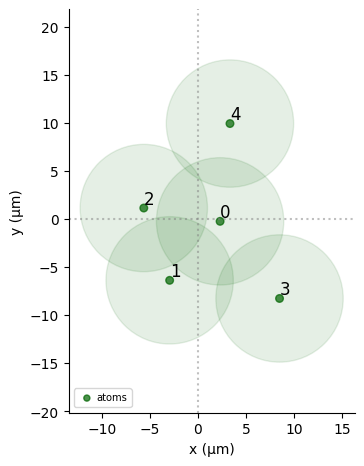
\includegraphics[height=7cm]{images/tutorials_qubo_14_0.png}    
\end{center}
\end{frame}



\begin{frame}{Moving the atoms to emulate QUBO}
We will use the \textit{Rydberg representation} of an hamiltonian by
\begin{itemize}
    \item we start is the state $H_I$ where $\Omega = 1 rad/{\mu s}$ and $\delta = 0 rad/{\mu s}$ 
    \item we end in the state $H_Q$ where  $\Omega = 0 rad/{\mu s}$ and $\delta = 1 rad/{\mu s}$ 
    \item we build parameterized \texttt{sequence} (Pulser experiment) to move slowly from $H_I$ to $H_Q$
\end{itemize}
\end{frame}

\begin{frame}[fragile]
\frametitle{Parameterized sequence}
\begin{verbatim}
LAYERS = 2

# Parametrized sequence
seq = Sequence(reg, DigitalAnalogDevice)
seq.declare_channel("ch0", "rydberg_global")

t_list = seq.declare_variable("t_list", size=LAYERS)
s_list = seq.declare_variable("s_list", size=LAYERS)

for t, s in zip(t_list, s_list):
    pulse_1 = Pulse.ConstantPulse(1000 * t, 1.0, 0.0, 0)
    pulse_2 = Pulse.ConstantPulse(1000 * s, 0.0, 1.0, 0)

    seq.add(pulse_1, "ch0")
    seq.add(pulse_2, "ch0")

seq.measure("ground-rydberg")    
\end{verbatim}
\end{frame}

\begin{frame}[fragile]
\frametitle{looping on sequences}
\begin{verbatim}
def quantum_loop(parameters):
    params = np.array(parameters)
    t_params, s_params = np.reshape(params.astype(int), (2, LAYERS))
    assigned_seq = seq.build(t_list=t_params, s_list=s_params)
    simul = QutipEmulator.from_sequence(assigned_seq, sampling_rate=0.01)
    results = simul.run()
    count_dict = results.sample_final_state()  # sample from the state vector
    return count_dict

np.random.seed(123)  # ensures reproducibility of the tutorial
guess = {
    "t": np.random.uniform(8, 10, LAYERS),
    "s": np.random.uniform(1, 3, LAYERS),
}    
example_dict = quantum_loop(np.r_[guess["t"], guess["s"]])


\end{verbatim}    
\end{frame}

\begin{frame}{looping on sequences and getting results}
A first run of function \texttt{quantum\_loop}, without optimisation, gets this resukt
\begin{center}
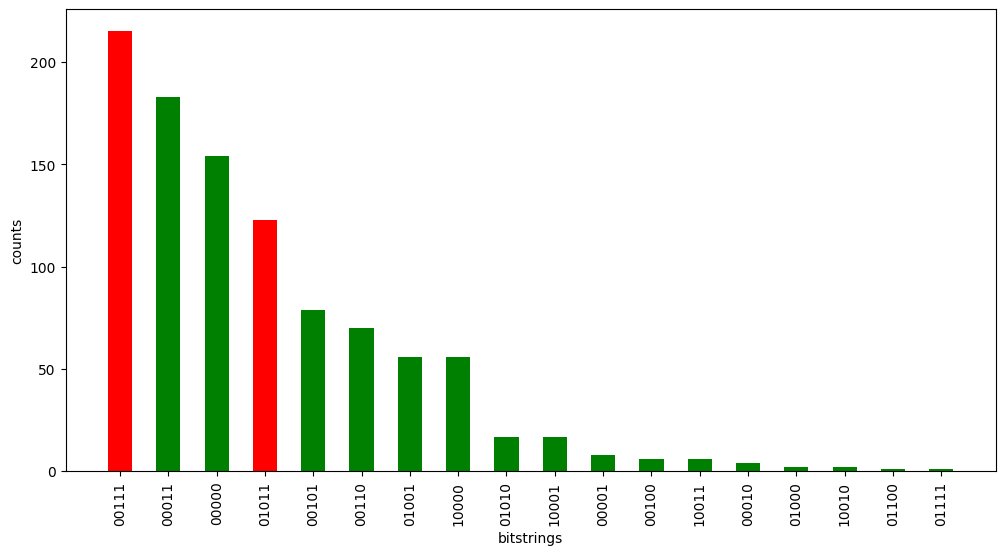
\includegraphics[width=8cm]{images/tutorials_qubo_27_0.png}    
\end{center}
We know that $01011$ and $00111$ are two minimal solution. We have not yet converged
\end{frame}

\begin{frame}[fragile]
\frametitle{Performing the optimisation}
A cost function \texttt{get\_cost}, computing $z^T.Q.z$ is define, it is fully polynomial. 

It it wrapped with  with \texttt{quantum\_loop}
\begin{verbatim}

def get_cost(counter, Q):
    cost = sum(counter[key] * get_cost_colouring(key, Q) for key in counter)
    return cost / sum(counter.values())  # Divide by total samples
    
def func(param, *args):
    Q = args[0]
    C = quantum_loop(param)
    cost = get_cost(C, Q)
    return cost    
\end{verbatim}
\end{frame}

\begin{frame}[fragile]
\frametitle{Invokation of the HPC optimizer}
\begin{verbatim}
scores = []
params = []
(...)
    try:
        res = minimize(
            func,
            args=Q,
            x0=np.r_[guess["t"], guess["s"]],
            method="Nelder-Mead",
            tol=1e-5,
            options={"maxiter": 10},
        )
        scores.append(res.fun)
        params.append(res.x)
(...)
\end{verbatim}    
\end{frame}


\begin{frame}{looping on sequences and getting results}
 
\begin{center}
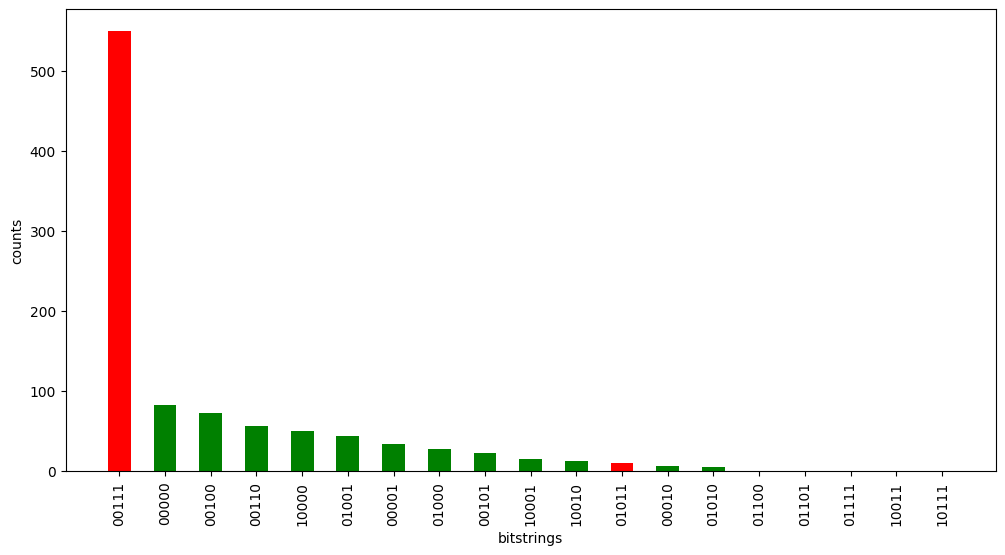
\includegraphics[width=8cm]{images/tutorials_qubo_38_0.png}    
\end{center}
Known solution are in red, we've found one, but thes second is still hidden. 
 
\end{frame}

\begin{frame}{The adiabatic theorem for dummies}
In Quantum Physics theory the adiabatic theorem says (roughly...)
\begin{itemize}
    \item a system is at the ground state of a system whose Hamiltonian $H_I$
    \item you make this system evolve continuously and \textit{kindly} to go to a configuration described by 
    hamiltonian $H_F$
    \item this evolution is \textbf{adiabatic}; no energy is brought to the system
\end{itemize}
Well... if you were nice enough with the system, you took it from $H_I$ in its ground state and put it $H_F$, at the 
ground state of $H_F$.

By measuring the state, you know what the ground state of $H_F$ is !!
This is (very roughly) how D-Wave machines operate. 
\newline
Let's build a sequence that make $\Omega$ and $\delta$ evolve adiabatically. 
\end{frame}


\begin{frame}[fragile]
\frametitle{Related Pulser code}
\begin{verbatim}
# We choose a median value between the min and the max
Omega = np.median(Q[Q > 0].flatten())
delta_0 = -5  # just has to be negative
delta_f = -delta_0  # just has to be positive
T = 4000  # time in ns, we choose a time long enough to ensure the propagation of information in the system

adiabatic_pulse = Pulse(
    InterpolatedWaveform(T, [1e-9, Omega, 1e-9]),
    InterpolatedWaveform(T, [delta_0, 0, delta_f]),
    0,
)
seq = Sequence(reg, DigitalAnalogDevice)
seq.declare_channel("ising", "rydberg_global")
seq.add(adiabatic_pulse, "ising")
seq.draw()
\end{verbatim}
\end{frame}
\begin{frame}{Adiabatic evolution}
We evolution of $\Omega$ and $\delta$ wavelengths will be design like this
\begin{center}
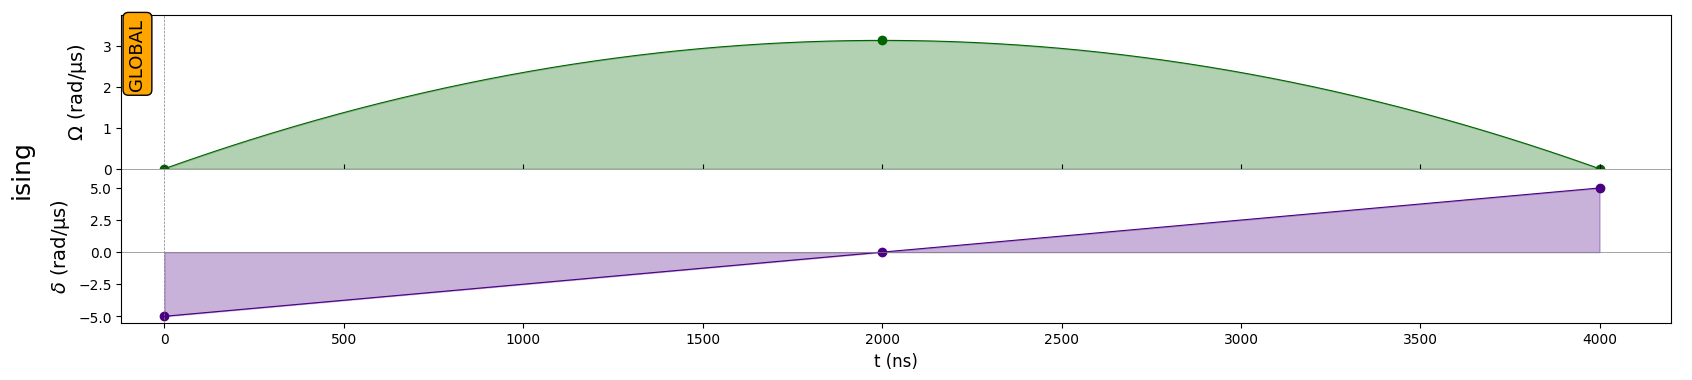
\includegraphics[width=14cm]{images/tutorials_qubo_46_0.png}    
\end{center}
\end{frame}

\begin{frame}{looping on sequences and getting results}
This time, we find both solutions in a very fast way 
\begin{center}
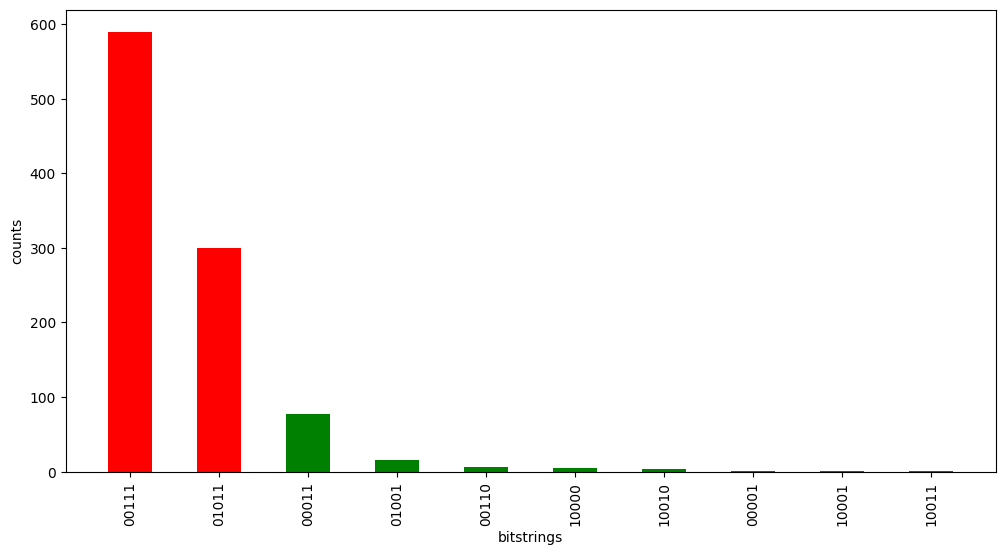
\includegraphics[width=8cm]{images/tutorials_qubo_48_0.png}    
\end{center}
It worked fine with this example, but building a $(\Omega, \delta)$ adiabatic evolution is complex.
 
\end{frame}
\section{Conclusion}

\begin{frame}{The paradox of the ancient modernity}
Quantum Computing seems to live it's early industrial time, but has old and solid basements
\begin{itemize}
    \item Quantum Physics is amost 100 years old
    \item the theory behind Quantum Computing is more than 30 years old
    \item but "actual" QPUs exist for less than 10 years
\end{itemize}
We should keep in mind that 
\begin{itemize}
    \item Quantum Computing is at the crossroad of recent technologies with an old theory behind the curtains
    \item even theory can be updated and enhanced
\end{itemize}
\end{frame}

\begin{frame}{Several technological axes}
Quantum Computing has several technological axes
\begin{itemize}
    \item different paradigms : QUANTUM GATES, annealers, analogic QPU, photonics
    \item different "qubits" : photons, supraconducting loops, cat qubits, ions trapped, neutral atoms...
    \item different contraints : cryogeny, lasers, maanagement of magnetic fields in the machine room
\end{itemize}
In this context
\begin{itemize}
    \item Which technologies will scale up to thousands of qubits?
    \item energy management is critical, some solution are even more expensive than HPC
\end{itemize}
Today, it's hard to tell which technologies or paradigms will survive beyond 10 years.
\end{frame}

\begin{frame}{Controversies}
Quantum Computing was almost ignored until the "rise" of Shor's algorithm. It holds many controversies
\begin{itemize}
    \item can QC brings a \textit{quantum advantage} or will HPCalways perform better than QC?
    \item are QC algorithms only "toys for mathematicians" or will they have concrete usages? Grover's algorithm is
    more specifically concerned.
    \item is "quantum gates" paradigm reliable in a long term perspective.
    \item are analogic QPU's capabilities structurally mimited?
    \item will QC replace HPC?
    \item Will QC change HPC? (as the \textit{quantum inspired} algorithm did)
\end{itemize}
\end{frame}

\begin{frame}{Lots of forthcoming changes}
As Quantum Computing evolves, many interesting aspects remain
\begin{itemize}
    \item at the hardware level (with lots of quantum physics))
    \item at the algorithmical level (with lots of mathematics)
    \item at the system software level as HPC/QC integration will require to modify HPC environments
    \begin{itemize}
        \item via impacts on users environments and programming environments
        \item via strong impact on scheduling policies and mechanisms
        \item via new services and compute methods provided to the end users
    \end{itemize}
    \item at the middleware level : almost nothing exists... most is still to be done
\end{itemize}
\end{frame}

\end{document}